\documentclass{article}
\usepackage{tikz} 
\usepackage{wrapfig}
\usepackage{amsmath} 
\usepackage[a4paper]{geometry}
\usepackage{fancyhdr}
\pagestyle{fancy}
\lhead{e und $\ln$ Funktion}
\rhead{März 2025}
\begin{document}
  
\section{Exponentialfunktion}
\subsection{Ableitungen}
Eine Exponentialfunktion kann abgeleitet werden, indem
\begin{enumerate}
 \item für $\dfrac{\mathrm{d}}{\mathrm{d}x} b^x = \ln{(b)} \cdot b^x$
 \item sie zu einer e-Funktion, welche einfach ableitbar ist, umgewandelt wird. Siehe unten 
\end{enumerate} 
 
\section{e-Funktion}
\begin{wrapfigure}{l}{5cm}
 \centering
 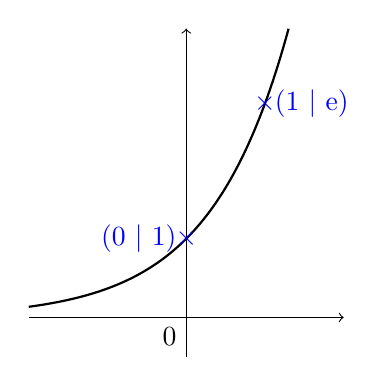
\begin{tikzpicture}     
  \draw[thick, domain=-2:1.3, samples=100] 
            plot (\x, {e^(\x)});
     
  \draw[->] (-2, 0) -- (2, 0); 
  \draw[->] (0, -0.5) -- (0, e^1.3);
 
  \draw (0, 0) node[below left] {0}; 
  \draw[blue] (0, 1) node {$\times$} node[left] {(0 $\vert$ 1)};
  \draw[blue] (1, e) node {$\times$} node[right] {(1 $\vert$ e)};
   
 \end{tikzpicture}
\end{wrapfigure}  
Eine e-Funktion ist eine Exponentialfunktion, welche die Eulersche Zahl $e \approx 2,718$ als Basis nimmt.
\[
 f(x)=e^x
\]
Somit ist sie in der Standardform streng monoton steigend und geht durch ${(0 \mid 1)}$, weil jegliche Zahl hoch null immer eins ist, und $(1 \mid e)$, weil $e^1=e$. \newline
Sie schmiegt bei im negativen an die x-Ache an, geht im positiven ins unendliche.
\[
 \lim_{x \to -\infty} e^x = 0
 \quad \text{und} \quad
 \lim_{x \to \infty} e^x = \infty
\]
Exponentialfunktionen anderer Basen können mit $a^x = e^{\ln{(a)} \cdot x}$ in eine e-Funktion umgewandelt werden. Dies folgt aus $a^x$ mit $a=e^{\ln{a}}$ und $(a^m)^n = a^{m \cdot n}$ 
\subsection{Ableitungen} 
Die Basis $e$ wird genutzt, um das Ableiten zu vereinfachen, es gilt $f(x)=e^x \implies f'(x)=e^x$. \newline
Beim Ableiten wird die Ableitung des Exponenten als Faktor vor das $e$ gesetzt, sodass 
\[
 \frac{\mathrm{d}}{\mathrm{d}x} e^{g(x)} = g'(x) \cdot e^{g(x)} 
\]  
\begin{wrapfigure}{r}{4.5cm}
 \centering
 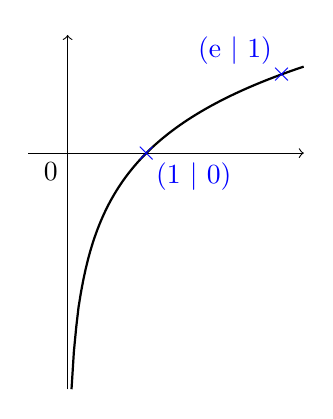
\begin{tikzpicture}     
  \draw[thick, domain=e^(-3):3, samples=100] 
            plot (\x, {ln(\x)});
     
  \draw[->] (-0.5, 0) -- (3, 0); 
  \draw[->] (0, -3) -- (0, 1.5);
 
  \draw (0, 0) node[below left] {0}; 
  \draw[blue] (e, 1) node {$\times$} node[above left] {(e $\vert$ 1)};
  \draw[blue] (1, 0) node {$\times$} node[below right] {(1 $\vert$ 0)};
   
 \end{tikzpicture}
\end{wrapfigure} 
Ist $g(x)$ eine lineare Funktion, kann das Gegenteil für das Bilden einer Stammfunktion genutzt werden. 
\[
 \int e^{mx+b} = \frac{1}{m} \cdot e^{mx+b}
\] 
\section{Natürliche Logarithmen}  
Der natürliche Logarithmus $\ln$ ist ein Logarithmus zur Basis $e$.
\[
 f(x) = \log_e{x} = \ln{x}
\] 
Somit ist die für $x>0$ definierte Standardform streng monoton steigend und geht durch ${(1 \mid 0)}$, weil jegliche Zahl hoch 1 gerechnet werden muss, um 0 zu bekommen, und $(e \mid 1)$, weil $e^1=e$. \newline
Sie schmiegt bei $x=0$ an die y-Ache an, geht im positiven ins unendliche.
\[
 \lim_{x \to 0^+} \ln x = -\infty
 \quad \text{und} \quad
 \lim_{x \to \infty} \ln x= \infty
\] 
Die Gegenfunktion zur e-Funktion, sodass $e^{\ln(m)}=\ln{(e^m)}=m$. Unteranderem daraus folgt auch dass $\ln(e)=1$.
\subsection{Ableitungen} 
\[
 \frac{\mathrm{d}}{\mathrm{d}x} \ln{(g(x))} = \frac{1}{g(x)} \cdot g'(x) 
\] 
\subsection{Integral}
$\ln{x}$ ist eine Stammfunktion zu $\dfrac{1}{x}$. Ist der Bruch nicht direkt in dieser Form gegeben, muss er in diese ausgeklammert werden, durch
\[
 \int \frac{a}{b \cdot x} =
 \int \frac{a}{b} \cdot \frac{1}{x} =
 \frac{a}{b} \cdot \ln(x)
\] 
 
\end{document}
 
 
 
 
